%!TEX root = skripsi.tex
%-----------------------------------------------------------------------------%
\chapter{\babDua}
%-----------------------------------------------------------------------------%

%-----------------------------------------------------------------------------%
\section{Pengenalan Entitas Kesehatan}
%-----------------------------------------------------------------------------%
% Apa itu MER
Pengenalan Entitas Kesehatan (\mer) merupakan salah satu cabang dari Pengenalan Entitas Bernama (NER) dengan dokumen sumber berupa teks kesehatan. NER sendiri merupakan suatu sistem/aplikasi yang memanfaatkan teknik pada \textit{Natural Language Processing} dan \textit{Information Extraction} untuk mengenali entitas yang telah dikategorikan sebelumnya seperti nama, lokasi, organisasi, waktu dll. Sedangkan pada sistem MER, entitas yang akan dikenali yaitu nama penyakit (\textit{disease}), gejala penyakit (\textit{sympton}), obat (\textit{drug}) dan langkah penyembuhan \textit{treatment}, nama protein, DNA, RNA dll. Gambar \ref{fig:mer_ilustration} merupakan ilustrasi dari sebuah sistem \mer.

% Contoh tentang MER
\begin{figure}
	\centering
	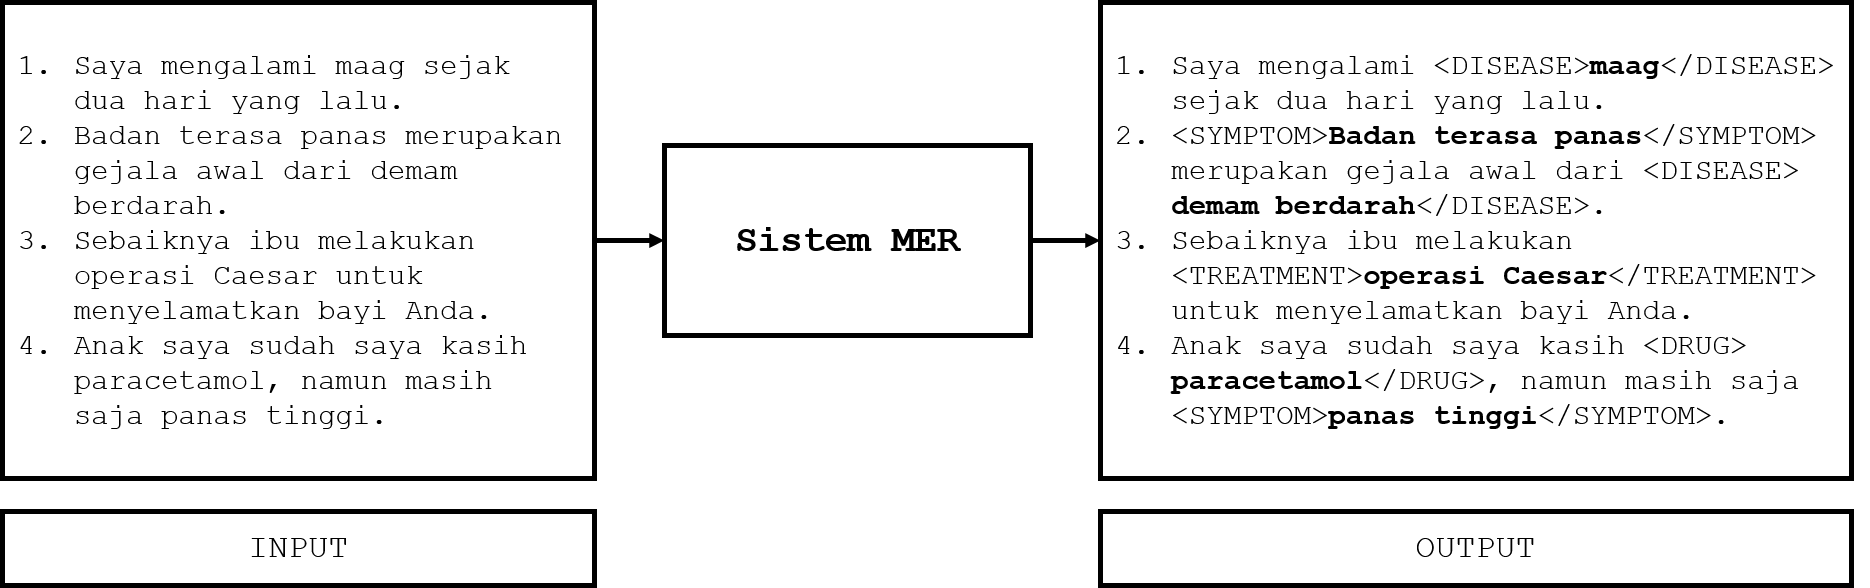
\includegraphics[width=1.0\linewidth]{images/mer_ilustration}
	\caption{Ilustrasi Sistem \mer}
	\label{fig:mer_ilustration}
\end{figure}

Dari ilustrasi di atas, sebuah sistem MER akan diberikan \textit{input} berupa dokumen kesehatan, kemudian sistem diharapkan dapat memberikan \textit{output} berupa dokumen yang mendapatkan pelabelan dengan benar. Dokumen kesehatan yang menjadi \textit{input} dapat berupa dokumen formal seperti dokumen suatu rumah sakit atau dokumen non-formal seperti dokumen forum kesehatan \textit{online}.

% Manfaat MER %
Implementasi sistem \mer~dapat memberikan manfaat pada beberapa bidang, seperti pada aplikasi \textit{Question Answering} \citep{abacha2011medical} yang hasil pelabelan dari sistem \mer~dapat mempermudah identifikasi entitas yang ditanyakan. Selain itu, hasil pelabelan sistem \mer~juga dapat dimanfaatkan untuk pembuatan sistem \textit{indexing} dokumen forum sehingga pencarian dokumen kesehatan dapat dilakukan dengan lebih efisien. Sistem \mer~juga dapat digunakan untuk mendukung aplikasi \textit{entity linking} yang memungkinkan seseorang untuk mengetahui hubungan antar entitas \citep{hachey2013evaluating}. Misalnya dengan adanya aplikasi \textit{entity linking}, kita dapat mengetahui obat apabila hanya diberikan \textit{query} nama penyakit dengan berdasarkan dokumen-dokumen kesehatan yang telah mendapatkan pelabelan dari sistem \mer. Masih banyak manfaat lain dari implementasi sistem \mer~ini.

% Cerita MER Bahasa Inggris %
Sebelumnya \cite{abacha2011medical} telah melakukan penelitian terkait sistem \mer~pada dokumen berbahasa Inggris. Sistem \mer~yang dibuat bertujuan untuk melabeli entitas \textit{treatment}, \textit{problem} dan \textit{test} dengan menggunakan 3 metode, yaitu (i) metode semantik dengan menggunakan \textit{tools} MetaMap (\textit{domain knowledge}), (ii) ekstraksi frasa berdasarkan \textit{chunker} dan klasifikasi dengan SVM (\textit{machine learning based}) dan (iii) gabungan 2 metode sebelumnya dengan menggunakan CRF (\textit{hybrid}). Hasil yang terbaik didapatkan dengan menggunakan metode \textit{hybrid} yang menggabungkan 2 metode sebelumnya (\textit{domain knowledge} dan \textit{machine learning}) dan dengan \textit{precision} $ 72.18\% $, \textit{recall} $ 83.78\% $ dan \textit{f-measures} $ 77.55\% $.

Selain penelitian di atas, \cite{mujiono2016new} juga melakukan penelitian terkait \mer~dengan tujuan untuk mendapatkan representasi data yang berdasarkan karakteristik \textit{training data}. \cite{mujiono2016new} mengusulkan tiga teknik representasi data, yaitu (i) evaluasi dengan model \textit{neural networsks} standar, (ii) evaluasi dengan dua \textit{deep network classifiers}, yaitu DBN (\textit{Deep Belief Networks}), dan SAE (\textit{Stacked Denoising Encoders}) serta (iii) representasi kalimat sebagai \textit{sequence} yang dievaluasi dengan \textit{recurrent neural networks} yaitu LSTM (\textit{Long Short Term Memory}). Hasil yang didapatkan yaitu kalimat sebagai \textit{sequence} yang dievaluasi dengan LSTM memberikan hasil yang terbaik, yaitu \textit{f-measure} $ 86.45\% $.

% Cerita MER Bahasa Indonesia (Kak Radit, Performa, Tabel) %
Penelitian terkait \mer~pada dokumen berbahasa Indonesia sudah dilakukan sebelumnya oleh \cite{skripsiKakRadit}. Dalam penelitiannya, \cite{skripsiKakRadit} menggunakan CRF (\textit{Conditional Random Fields}) dengan tujuan untuk mendapatkan kombinasi fitur yang menghasilkan akurasi terbaik. Entitas yang akan diberi label yaitu nama penyakit (\textit{disease}), gejala penyakit (\textit{sympton}), obat (\textit{drug}) dan langkah penyembuhan \textit{treatment}. Dokumen yang menjadi input penelitian merupakan hasil \textit{crawling} dari  forum kesehatan \textit{online} dari berbagai situs yang berisi tanya jawab. Hasil yang didapatkan yaitu \textit{precision} $ 70.97\% $, \textit{recall} $ 57.83\% $ dan \textit{f-measeure} $ 63.69\% $ dengan fitur \textit{its own word}, frasa, kamus (\textit{symptom}, \textit{disease}, \textit{treatment} dan \textit{drug}), kata pertama sebelum dan panjang kata.

Selain itu, \cite{suwarningsih2014imner} juga melakukan penelitian terkait \mer~pada dokumen berbahasa Indonesia dengan menggunakan SVM (\textit{Support Vector Machine}). Entitas yang akan dikenali yaitu \textit{location}, \textit{facility}, \textit{diagnosis}, \textit{definition} dan \textit{person}. Data yang digunakan sebagai korpus merupakan data dari situs \textit{health.detik.com}, \textit{detikhealth.com} dan \textit{health.kompas.com/konsultasi} dengan total keseluruhan sebanyak 1000 kalimat. AKurasi yang dihasilkan yaitu $ 90\% $ dengan menggunakan fitur \textit{baseline}, \textit{word level (morphology, POS-Tag, dll)} dan fitur dari dalam dokumen tersebut.

\section{Deep Learning}
--Belum

\section{Recurrent Neural Networks}\label{sec:rnns}

\textit{Recurrent neural networks} (RNNs) merupakan \textit{Artificial Neural Networks} (ANNs) yang memiliki koneksi siklik \citep{graves2012neural}. RNNs memiliki \textit{neuron} yang terkoneksi dengan \textit{neuron} lain sehingga membentuk \textit{loop} umpan balik (\cite{haykin2009neural}), tidak seperti \textit{feedforward neural network} (FNNs) dimana aliran informasi hanya berjalan searah. RNNs memungkinkan \iob~yang dihasilkan akan menjadi \ioa~untuk menghasilkan \iob~yang lain. Hal ini menyebabkan perilaku RNNs tidak hanya bergantung pada \ioa~saat ini saja, namun juga bergantung pada \iob~sebelumya. Oleh karena itu, RNNs memiliki kemampuan yang sangat bagus sebagai model dalam permasalahan \textit{sequence data} dibandingkan dengan FNNs. RNNs sendiri memiliki kemampuan yang sangat bagus dalam beberapa \textit{task}, seperti \textit{language model} (\cite{mikolov2010recurrent}) dan \textit{speech recognition} (\cite{graves2013speech}).

Dibandingkan dengan FNNs, RNNs memiliki beberapa kelebihan \citep{mikolov2010recurrent}, yaitu:
\begin{enumerate}
	\item Pada RNNs, kata-kata sebelumnya direpresentasikan dengan \textit{recurrent connections}, sehingga RNNs dapat menyimpan informasi kata sebelumnya dalam jumlah tak hingga. Pada FNNss, representasi kata sebelumnya berupa konteks dari n-1 kata. Oleh karena itu, FNNs terbatas dalam penyimpanan informasi kata sebelumnya terbatas seperti pada model n-gram.
	\item RNNs dapat melakukan kompresi keseluruhan riwayat kata menjadi ruang dimensi yang lebih kecil, sedangkan FNNs melakukan kompresi/proyeksi hanya dengan sebuah kata saja.
	\item RNNs memiliki kemampuan membentuk \textit{short term memory}, sehingga dapat posisi invarian sebuah kata dapat ditangani. Hal ini tidak dapat dilakukan pada FNNs,
\end{enumerate}

Banyak variasi RNNs yang telah diusulkan oleh beberapa peneliti, seperti Elman \textit{networks} \citep{elman1990finding}, Jordan \textit{networks} \citep{jordan1986attractor}, \textit{time delay neural networks} \citep{lang1990time} dll. Gambar berikut merupakan conroh  dari RNNs sederhana

\begin{figure}
	\centering
	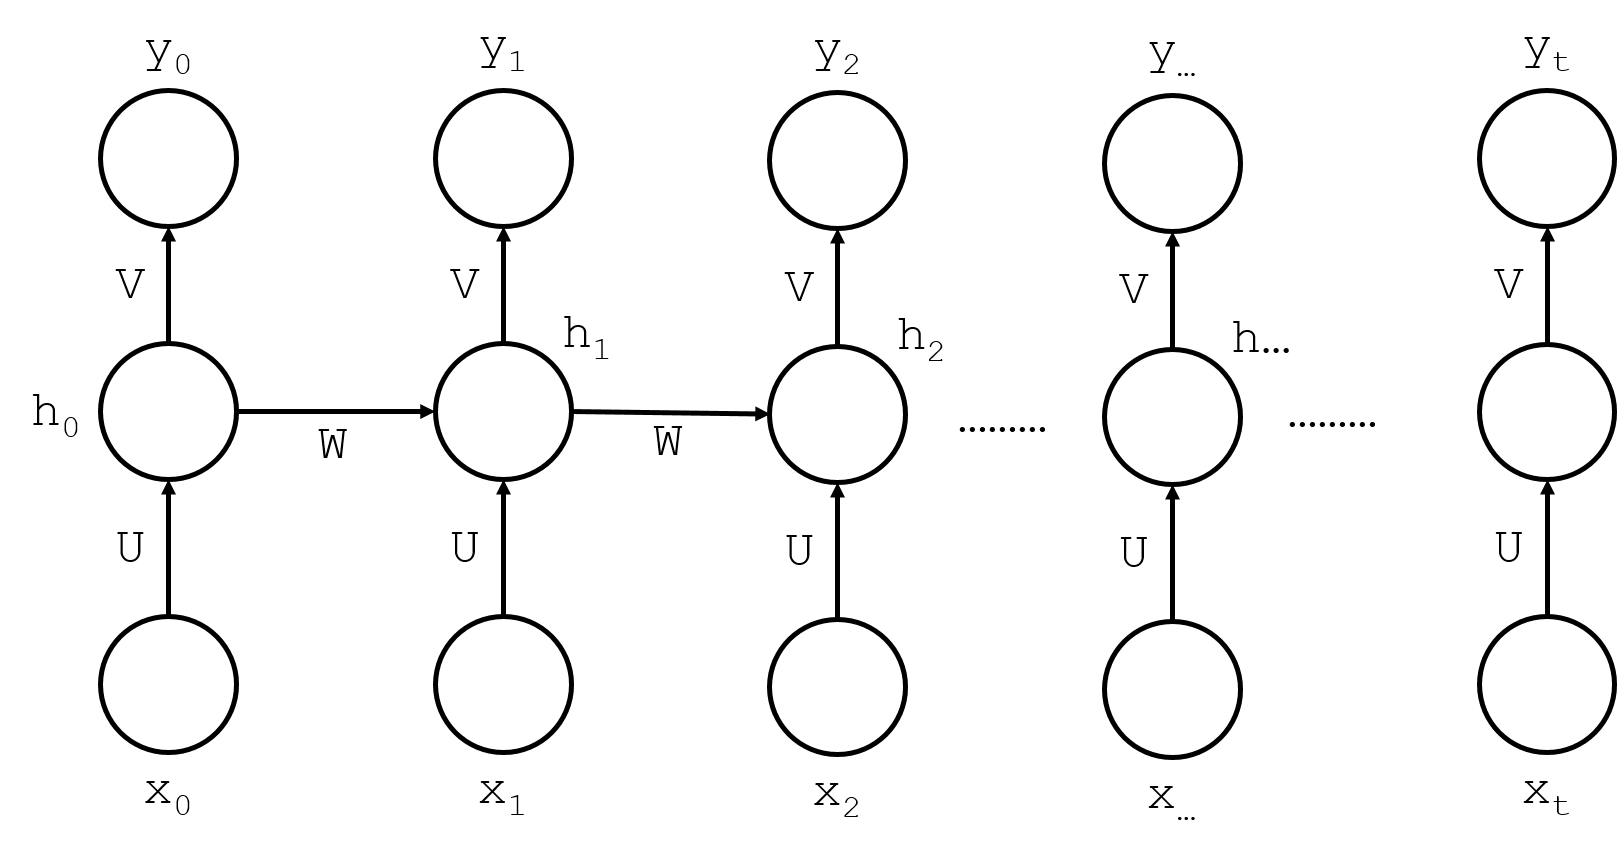
\includegraphics[width=0.80\linewidth]{images/simple_rnn}
	\caption{\textit{Recurrent Neural Networks} sederhana}
	\label{fig:simple_rnn}
\end{figure}

Dari gambar \ref{fig:simple_rnn}, sebuah jaringan pada RNNs memiliki \textit{input layer} $ x $, \textit{hidden layer} $ h $ dan \textit{output layer} $ y $. Terdapat 3 buah parameter yang dicari dalam tahap \textit{learning}, yaitu $ {U, V, W} $ yang masing-masing parameter tersebut di-\textit{share} untuk semua \textit{timestep} $ t $ dengan:
\begin{equation}\label{equ:euclideandistance}
U, V, W \in {\rm I\!R}
\end{equation}

Untuk suatu \textit{timestep} $ t $, \textit{input} RNNs dinotasikan sebagai $ x(t) $, \textit{timestep} dinotasikan sebagai $ h(t) $ dan \textit{output} dinotasikan sebagai $ y(t) $, dengan:
\begin{equation}
y(t) = f(V \cdot h(t))
\end{equation}
\begin{equation}
h(t) = f(U \cdot x(t) + W \cdot h(t-1))
\end{equation}
dimana
\begin{equation}
h(0) = f(W \cdot x(0))
\end{equation}
dengan $ f $ sebagai \textit{activation function}. Untuk lebih jelasnya, berikut merupakan gambar dari satu buah \textit{timestep} di dalam RNNs
\begin{figure}
	\centering
	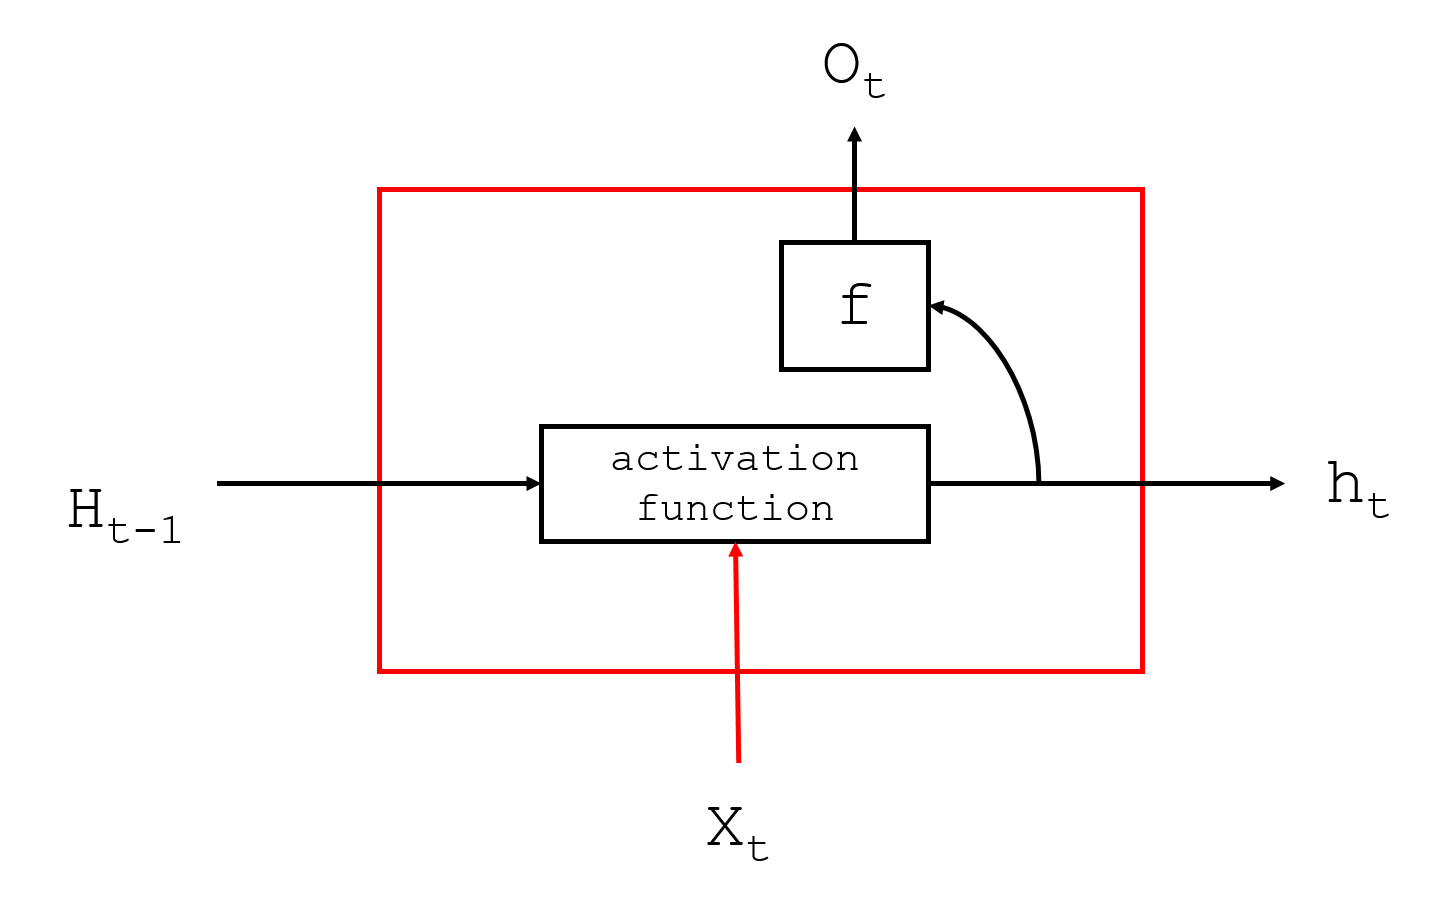
\includegraphics[width=0.80\linewidth]{images/nodes_rnn}
	\caption{1 buah \textit{timestep} dalam RNNs}
	\label{fig:nodes_rnn}
\end{figure}

\subsection{Long Short Term Memory}
Pada penjelasan di atas, RNNs memiliki kelebihan mempertimbangkan konteks untuk mengolah \textit{input} menjadi \textit{output}. Sayangnya, \textit{range} konteks yang dapat digunakan dalam satu blok terbatas \citep{graves2012neural}. Efek dari keterbatasan ini yaitu informasi pada suatu blok akan hilang atau terganggu dengan konteks sebelumnya sehingga \textit{output} yang dihasilkan tidak sesuai harapan. Ilustrasi masalah yang disebut \textit{vanishing gradient problem} ini dapat dilihat di FIGUREX. Banyak upaya untuk mengatasi masalah ini, seperti dengan menggunakan \textit{simulated annealing} dan \textit{discrete error propagation}, menggunakan \textit{time delays} atau \textit{time constant}, dan \textit{hierarchical sequence compression}. Namun sejauh ini solusi yang paling bagus yaitu dengan arsitektur \textit{Long Short Term Memory} (LSTM).

\subsection{Penerapan RNNs untuk MER}
-- Belum

\section{Word Embedding}
-- Belum
%-----------------------------------------------------------------------------%
% Cerita umum Word Embedding terlepas dari, kenapa bukan %
% Salah satunya adalah word2vc%
% CBOW vs Skip %
